\paragraph{API Handling}

The \ac{API} handling is an essential part of the chatbot system, providing interaction between the frontend and the
backend. The \ac{API} connects various services, such as case management, message sending, and supplier handling, to
ensure that the system operates seamlessly. This section covers on one side the most important functions from the
\texttt{api.ts}, \texttt{v1.json}, and \texttt{v1.d.ts} files, which define the \ac{API}'s structure, types, and
requests. On the other side, there are three composables in the project that play a significant role in facilitating
\ac{API} interactions: \texttt{useApiClient.ts}, \texttt{useCasesApi.ts}, and \texttt{useMessagesApi.ts}. These
composables encapsulate \ac{API}-related logic, making it easier to reuse and manage the interactions between the
frontend and the backend.

The \texttt{api.ts}
file defines core types and utilities that are crucial for \ac{API} interactions. It leverages TypeScript's type system
to define \ac{API} schema models, ensuring that all requests and responses are strongly typed and consistent throughout
the application.

The following snippet defines the types for \texttt{Case}, \texttt{State}, and \texttt{Message}, as shown in Code
\ref{lst:api-core-types}.

% @formatter:off
\begin{lstlisting}[language=JavaScript, caption={Core API Types (\texttt{api.ts})},
  firstnumber=1,label={lst:api-core-types}]
export type Case = components['schemas']['Case']
export type State = ArrayType<NonNullable<components['schemas']['Case']['state']>>
export type Message = components['schemas']['Message'] & {
  loading?: boolean
}
\end{lstlisting}
% @formatter:on

The \texttt{Case}, \texttt{State}, and \texttt{Message} types are derived from the OpenAPI schema (defined in the
\texttt{v1.json} file). These types ensure that every interaction with the \ac{API} adheres to the structure
defined by the backend. The \texttt{Message} type is extended to include a \texttt{loading} property
, allowing the frontend to track when a message is being processed, providing better feedback to the user.

The \texttt{v1.json} file represents the OpenAPI schema forthe backend. It defines all available \ac{API} endpoints,
their parameters, and their expected responses. This structure is crucial for understanding how the frontend interacts
with the backend.

Code \ref{lst:api-v1-json}, stored in \ref{subsec:frontend}, defines the \texttt{/api/v1/cases} endpoint for listing and
creating cases.

This endpoint supports both listing (GET) and creating (POST) cases. The GET method allows
filtering by \texttt{user\_id} and limiting the number of cases retrieved. The POST method requires a
\texttt{CreateCaseRequest} body to create a new case.
Each operation has a unique \texttt{operationId} (e.g., \texttt{list\_cases\_api\_v1\_cases\_get}), which is
used to reference and document the \ac{API} call.

Because OpenAPI is used, the \ac{API} Endpoints can be shown in the schema from Swagger as shown in Figure
\ref{fig:swaggerui}.

\begin{figure}[H]
\centering
\caption[Swagger UI]{Swagger UI \footnotemark}
\label{fig:swaggerui}
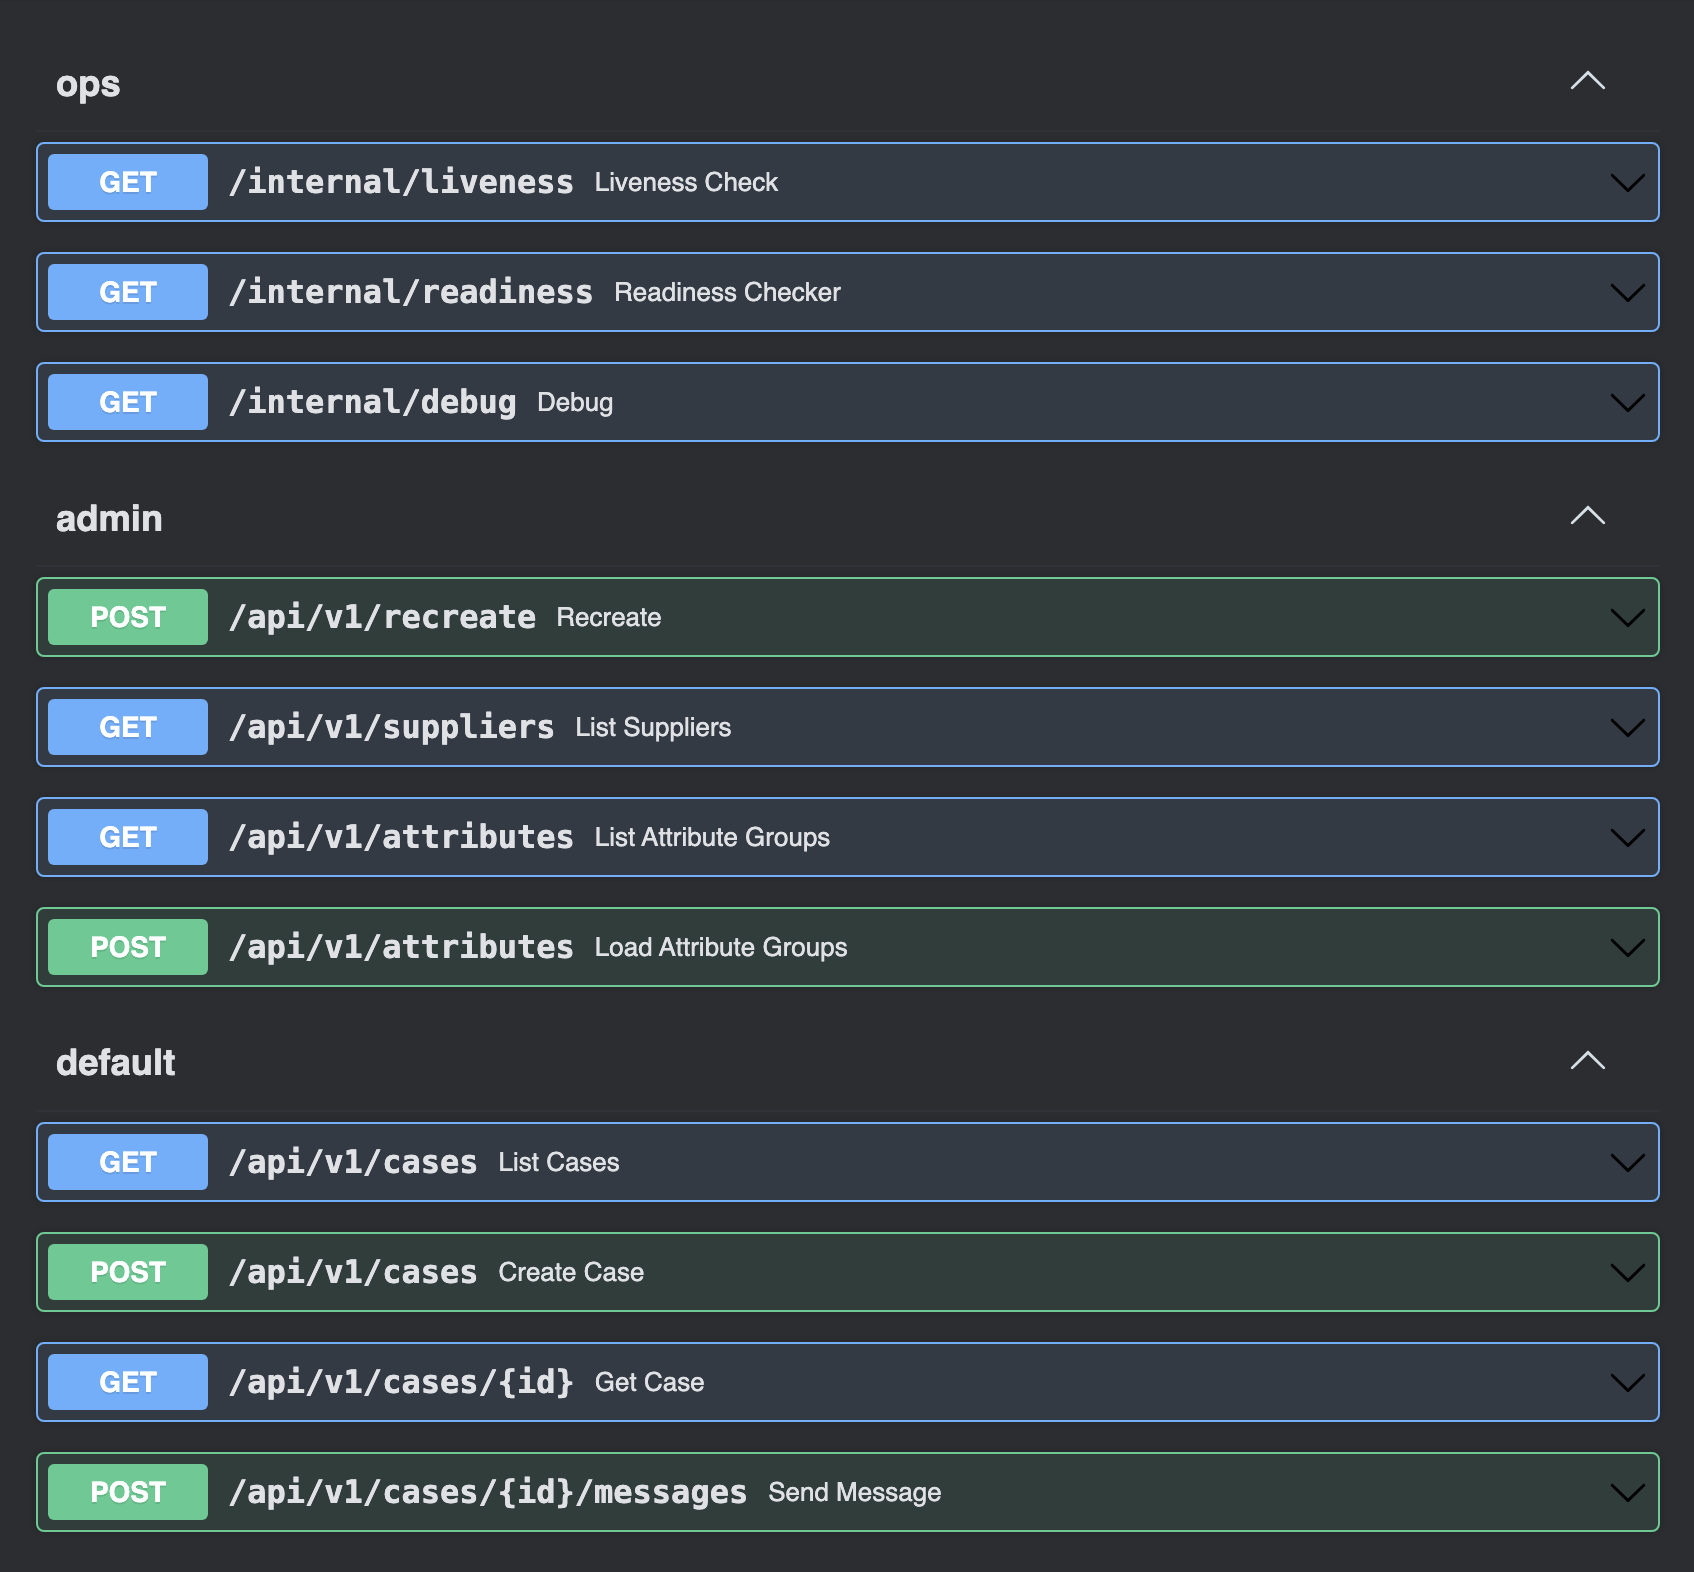
\includegraphics[width=1\textwidth]{abbildungen/Prototyping/Swagger_UI.png}
\end{figure}
\footnotetext{Own illustration}

This made it easy to test the \ac{API} Endpoints without implementing them directly in the code.

The \texttt{v1.d.ts} file defines the TypeScript types generated from
the OpenAPI schema, ensuring that all \ac{API} requests and
responses are typed correctly. This provides strong typing for all
interactions with the \ac{API}, helping prevent runtime errors and ensuring that the frontend and backend stay in sync.

The following snippet shows the type definition for the \texttt{Case} schema, as demonstrated in Code
\ref{lst:case-schema}.

% @formatter:off
\begin{lstlisting}[language=JavaScript, caption={Case Schema Definition (\texttt{v1.d.ts})},
  firstnumber=260,label={lst:case-schema}]
export interface components {
  schemas: {
    Case: {
      /**
      * Id
      * Format: uuid
      */
      id: string;
      /** State */
      state?: components["schemas"]["StateAttributeGroup"][];
      /** Messages */
      messages?: components["schemas"]["Message"][];
      /**
      * Created At
      * Format: date-time
      */
      created_at: string;
      /** Title */
      title?: string | null;
      case_type?: components["schemas"]["SystemCaseTypeEnum"] | null;
    };
  }
}
\end{lstlisting}
% @formatter:on

This schema defines the structure of a \texttt{Case} object, which includes fields such as \texttt{id
}, \texttt{state}, \texttt{messages}, \texttt{created\_at}, and optional fields like \texttt{title} and \texttt{
case\_type}. The \texttt{state} field contains an array of \texttt{StateAttributeGroup} objects
, while the \texttt{messages} field contains an array of \texttt{Message} objects, demonstrating the
complexity of the data model.

The \texttt{useApiClient.ts} file defines a function that sets up and returns an \ac{API} client. It uses the
\texttt{openapi-fetch} library to create a client that
interacts with the defined OpenAPI schema. The client is configured with a base URL, and headers can be added
as needed. This client serves as the primary way to make \ac{API} calls throughout the application.

Code \ref{lst:use-api-client} demonstrates how the \texttt{useApiClient} function is defined.

% @formatter:off
\begin{lstlisting}[language=JavaScript, caption={Setting up the API Client (\texttt{useApiClient.ts})},
  firstnumber=4,label={lst:use-api-client}]
export const useApiClient = () => {
  return createClient<paths>({
    baseUrl: import.meta.env.VITE_API_BASE_URL,
    headers: {
      // Authorization: `Basic ${import.meta.env.VITE_API_CREDENTIALS}`
    }
  })
}
\end{lstlisting}
% @formatter:on

The \texttt{useApiClient} function encapsulates
the configuration of the \ac{API} client, allowing other composables to easily import and use it. This approach keeps
the \ac{API} setup centralized and manageable, making it easy to configure base URLs and headers in one place.

The \texttt{useCasesApi.ts} file defines the composable for interacting with
cases-related \ac{API} endpoints. It utilizes the \ac{API} client to fetch and create cases and employs
\texttt{vue-query} for managing data caching, mutation, and state.

The following snippet shows how the \texttt{findAll} function is implemented using \texttt{vue-query}, as demonstrated
in Code \ref{lst:use-cases-api-findall}.

% @formatter:off
\begin{lstlisting}[language=JavaScript, caption={Fetching All Cases (\texttt{useCasesApi.ts})},
  firstnumber=19,label={lst:use-cases-api-findall}]
const findAll = useQuery({
  queryKey: ['cases'],
  queryFn: async () => {
    return (
      await client.GET('/api/v1/cases', {
        params: {
          query: {
            user_id: userStore.userId
          }
        }
      })
    ).data?.cases
  },
  ...defaultQueryOptions
})
\end{lstlisting}
% @formatter:on

This function uses \texttt{vue-query} to fetch all cases for a specific user.
It defines a \texttt{useQuery} with a unique \texttt{queryKey} (\texttt{['cases']}) and a \texttt{queryFn} that performs
a GET request to the \texttt{/api/v1/cases} endpoint, passing the user's ID as a query parameter. The
default options are applied to the query to manage retry behavior and error handling.

The \texttt{useCasesApi} composable also includes functions for creating a case and fetching a
case by its ID. It leverages Vue's reactivity to make
these operations seamless within the application, allowing components to respond automatically to changes in the data.

The \texttt{useMessagesApi.ts} file defines the composable for interacting with message-related
\ac{API} endpoints. It primarily handles sending messages for a given
case and fetching the list of messages. Similar to \texttt{useCasesApi.ts}, this composable uses the shared \texttt
{useApiClient} and integrates with \texttt{vue-query} for data management.

The \texttt{create} function in \texttt{useMessagesApi} sends a new message to the
backend by making a POST request to \texttt{/api/v1/cases/\{id\}/messages}, with the message content
as the request body. This function allows the chatbot to send user-generated messages and system messages effectively.

The composable \texttt{useMessagesApi.ts} also includes a \texttt{findAll} function to fetch all
messages associated with a specific case. This function is accomplished
by extending the \texttt{findById} method from \texttt{useCasesApi}, ensuring consistency in handling \ac{API}
interactions across the project.
